\section{Hotel Daten von vielen Hotels}
\label{sec:all_Hotels}
Das Konzept \emph{Hotel Daten von vielen Hotels} verfolgt die grundlegende Idee, sämtliche bis dato gesammelten Hoteldaten zu konsolidieren und ein umfassendes, übergeordnetes Modell des maschinellen Lernens zu entwickeln.
\newline
\newline
Die bereits vorhandenen Daten aus zahlreichen Hotels bildet die Basis für den Aufbau eines solchen Modells. Dieses Vorhaben sieht vor, das bereits existierende RevPAR-Modell zu modifizieren und zu erweitern. Zunächst wird angestrebt, alle Hotels in eine vergleichbare Form zu bringen. Eine mögliche Herangehensweise hierbei ist die Definition bestimmter Hotelmerkmale und ihre Auflistung als Vektor, um eine Vergleichbarkeit zu ermöglichen.
\newline
\newline
Im nächsten Schritt ist eine Anpassung des RevPAR-Modells erforderlich, da dieses normalerweise auf Buchungsdaten basiert. Für Hotels ohne historische Buchungsdaten ist es offensichtlich nicht möglich, diese als Features zu verwenden, da sie schlichtweg nicht verfügbar sind. Stattdessen sollen die charakteristischen Merkmale jedes Hotels dem jeweiligen RevPAR zugeordnet werden.
\newline
\newline
Sobald das RevPAR-Modell entsprechend umstrukturiert ist, können sämtliche Hotels in der Datenbank als Datensätze dem Modell zugeführt werden. Falls ein Hotel ohne vergangene Buchungsdaten auftaucht, können basierend auf seinen charakteristischen Eigenschaften Prognosen über den zu erwartenden RevPAR getroffen werden. In diesem Szenario muss das Hotel lediglich, wie alle anderen Hotels auch, eine Zuordnung zwischen dem RevPAR und dem tatsächlichen Preis festlegen.
\newline
\newline
Die Aufmachung dieses Konzeptes soll im folgenden Schaubild nochmal Bildlich verdeutlicht werden:
\begin{figure}[h]
    \centering
    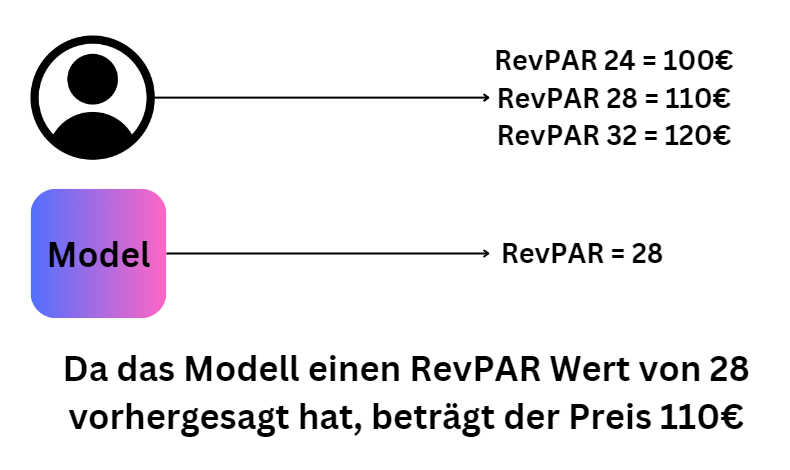
\includegraphics[width=0.5\textwidth, center]{RevPAR_all.png}
    \caption[RevPAR-Modell Vorgehen]{RevPAR-Modell Vorgehen}
    \label{img:all_hotels}
\end{figure}

Dieser Ansatz zielt darauf ab, eine umfassende Verwendung der vorhandenen Daten zu ermöglichen und somit auch für Hotels ohne historische Buchungsdaten eine Prognose des RevPAR auf der Grundlage ihrer individuellen Eigenschaften zu ermöglichen.